\section{Concept 2 - Component/structure editor}
The second concept originated from the idea that structure, could be added by component-based tool. Hiding some of the complexity of the constrains of a data model behind a simple user interface supplying dragable components and providing immediate visual feedback in the form of textual use case representation (or a diagram) could "cheat" the customer into adding the needed structure to the use case model.

Concept is to define everyhing beforehand, and create use cases from these predefined actors, actions and concepts.

An example UI is Starting from scratch, the user would be expected to initially define at least one actor and add a sequence of actions that the actor perform.


A big problem with this approach is that it could quickly lead to artificial or too technical jargon in use cases, which is generally a bad idea as it alienates the customer \cite{christel1992}.


\begin{figure}[!htbp]
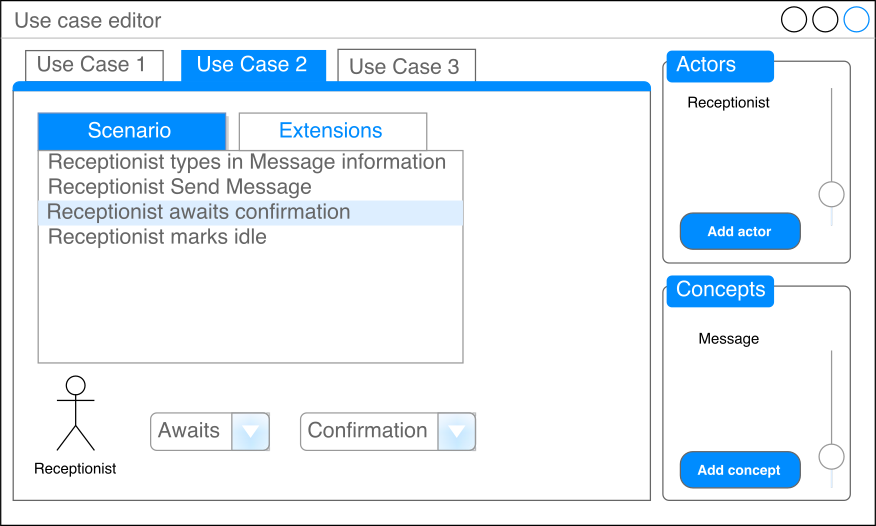
\includegraphics[scale=0.9]{img/test_case_ui}
\centering
\caption{Use case editor UI mockup}
\label{fig:use_case_editor_mockup}
\end{figure}

\section{Interpreting use cases}
%IN SUMMARY; How much information can you acutally derive from a use case?
%A use case scenario should always terminate.

This section tries to extracts an abstract interpretation of a use case through a brief study of two use cases. The goal is to come up with a meta-model of use cases that captures the essentials of the informally written use case, and allow us to map the concepts from it to an abstract syntax so that test code may be generated from it.

The first use case is a basic phone call forwarding session that goes though a receptionist. The use case is described from the receptionist's point of view, as this is the scope of the main case study system. The use case has a detailed description in schema form in figure \ref{fig:uc1}. \\\\
The second use case is, in a sense, embedded in the first one as it part of the extensions of that use case. This will be covered later on. The use case covers a ``send message'' session typically done by having the receptionist actor transcribe a spoken message along with caller information (name, company, ...) onto a set of text input fields that then can be assembled to a message. This message is then handed over to the system that may enqueued it for later delivery -- or send it immediately, depending on implementation.

\subsection{Identifying concepts}
The first concept we know, for certain, should got into our meta model is the use case. It serves as our top-level concept that every other concept, in some way, relates to. From here on, we go back to our two case study use cases use cases where we can easily -- by manual inspection -- identify various concepts that most likely also belongs in a domain model. In use case 1 (figure \ref{fig:uc1}), we see three different actors: A receptionist, a contact and a caller. We also have a primary actor that provides us with the ``glasses'' we see the use case through. This, in conclusion, means that we need an actor as part of our domain model, and an association between a use case and an actor.\\\\
Skipping the pre- and postconditions for now, we take a look at the ``Main success scenario'' and see that, broadly speaking, each use case action involves one actor performing an action, possibly affecting a target object -- which could be another actor. For the purpose of generating tests, it is not important that actors may target other actors though their actions, and this association is therefore left out of the meta model.\\\\
Given the loose structure of the use case concept, we believe it is sufficient to treat preconditions as simply other use cases. A more elaborate motivation for this can be found in section \ref{sec:test_case_state}.\\\\
Postconditions are defined to be predicates. This is because they share the common trait that they must be true, for the given expression to be true. In our case, the postcondition ``Receptionist is ready for next call'' states the actor receptionist that is participating in this use case, must be in a specific state when the last statement of the use case is done. A postcondition should refer to an actor, target or action previously defined in the use case to avoid redundant mapping. The predicate itself can be some sort of quantifiable strict logic such as ``Message has recipients'', or could as an extension be defined as the more loose ``Message should have recipients'', which should map to a warning in the generated tests, rather than an error.

Pre and post-conditions are operations that work on expressions rather than statements

Alternate scenarios are not yet covered.

\subsection{Meta model}
This section contains a brief discussion of a meta model that could be used for translating use cases into test cases. The discussion is supported by the graphical model depicted in figure \ref{fig:meta_model}\\\\
Within the definition mapping, the mapping class denotes the relation between either a predicate and a predicate expression, or a statement (indirectly by the actor, action, target composition). The mapping is uniquely defined by mapping by its composition of an actor, an action and a target, as it should be safe to assume that ``The contact accepts the call'' means the same no matter which use case it appears in. Each mapping will imply a requirement on a resource, which can be any actor or target. The are basically constraints stating the minimum functionality the test framework\footnote{Domain-specific scaffolding code that needs to be written by hand} should have to make the generated test code runnable. These resources could, in test code frameworks, be provided by factory classes or object pools.\\\\
Tests are the output of a sequence of mappings, that has a state which is then defined by the mappings that originally defined the test. The test will also have references to the predicate expressions that are outputted by mappings as well.

\begin{figure}[h]
  \centering
 
  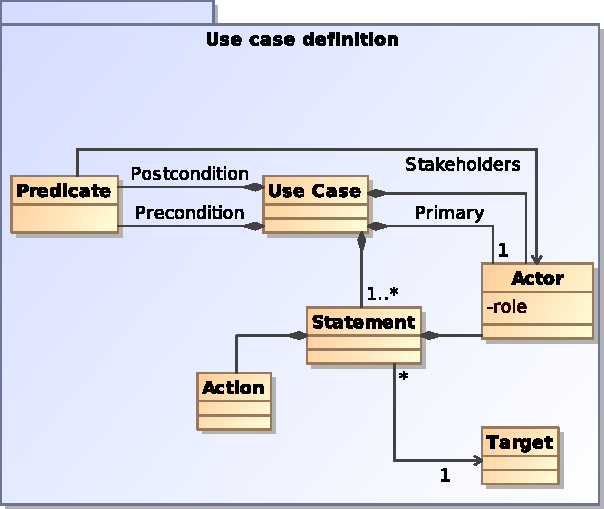
\includegraphics[scale=0.72]{img/use_case_meta_model}
  \caption{Intermediate meta model for use case representation along with tests}
  \label{fig:use_case_meta_model}
\end{figure}

\begin{figure}[h]
  \centering
 
  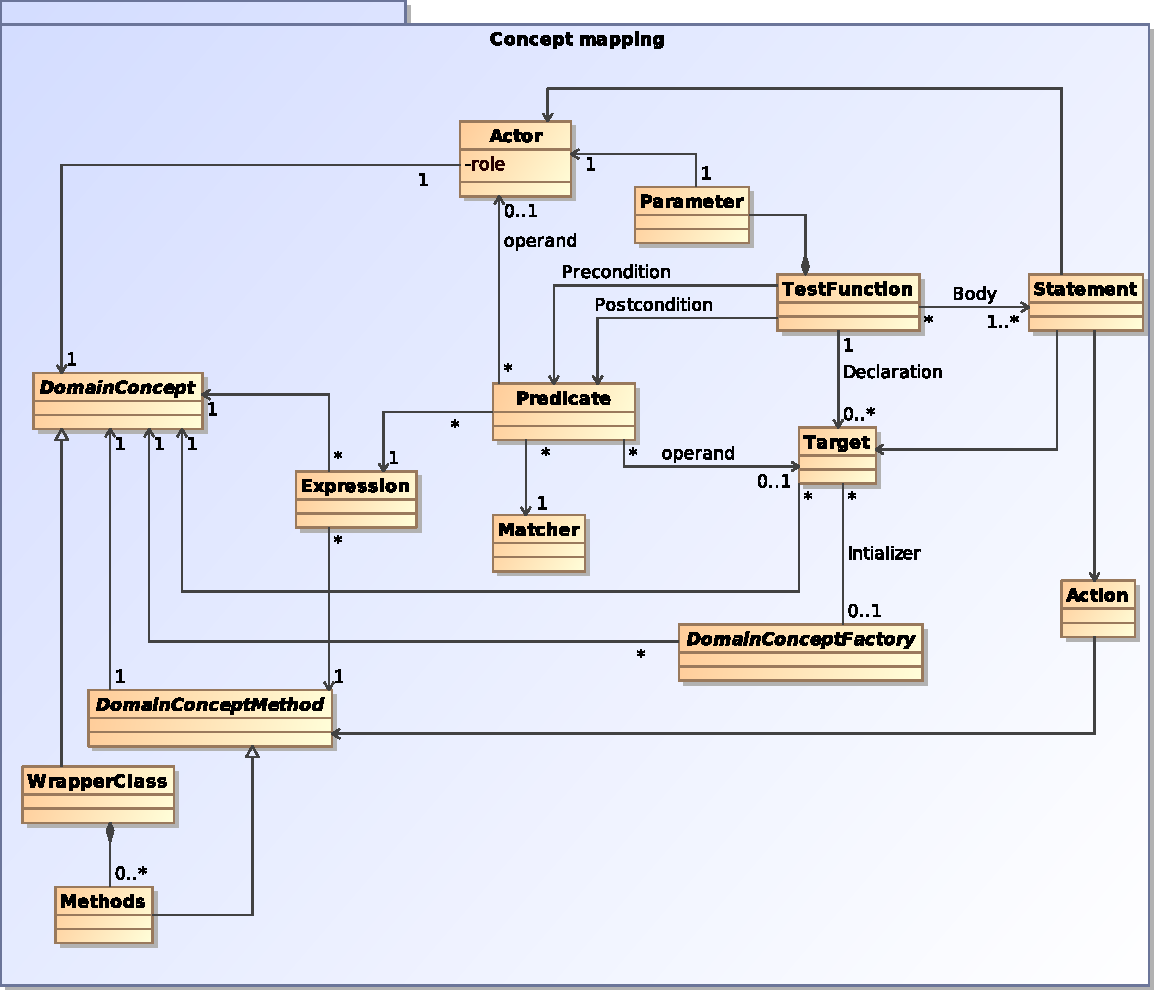
\includegraphics[scale=0.72]{img/use_case_mapping}
  \caption{Use case mapping}
  \label{fig:use_case_mapping}
\end{figure}

\section{Mapping manually}
Within a use case there are some bits of implicit knowledge that we need to extract. To begin with, we observe that for the use cases in figure \ref{fig:uc1} and \ref{fig:uc2}, there are domain actors involved.

Each involved domain actor will then be mapped to a wrapper class that represents the domain object, and could possibly extend a class from the implemented code base.

In order to get the actor object to perform actions, we need to map the actions in the use case to some functions associated with the actor class. These functions could be a direct link to a method that is part of the main codebase which is tested against, a new method written specifically for this purpose - or a macro function that combines functionality from different domain concepts in a single functions.

Whenever there is a mention of an object (a target of an action) which could be, for instance, a message object we assume that its the same object that is tracked during the entire use case. So, from use case 2, we have ``Receptionist sends the message via the system'' in the main success scenario and ``Message is stored and ready for dispatching'' in the postconditions.

So, summing up, we have in this model a very strict view on single use case entries:
\begin{itemize}
  \item This use case consists of an ordered list of actions, where actions consist of
  \begin{itemize}
	\item One or more actors
	\item One verb describing the action
	\item One target for the action (object for verb)
  \end{itemize}
\end{itemize}
If we 


One of the problems with this solution is that you also need to specify who is performing the action, and who is the target.
